% Options for packages loaded elsewhere
\PassOptionsToPackage{unicode}{hyperref}
\PassOptionsToPackage{hyphens}{url}
%
\documentclass[
  american,
  man,floatsintext]{apa7}
\usepackage{amsmath,amssymb}
\usepackage{lmodern}
\usepackage{ifxetex,ifluatex}
\ifnum 0\ifxetex 1\fi\ifluatex 1\fi=0 % if pdftex
  \usepackage[T1]{fontenc}
  \usepackage[utf8]{inputenc}
  \usepackage{textcomp} % provide euro and other symbols
\else % if luatex or xetex
  \usepackage{unicode-math}
  \defaultfontfeatures{Scale=MatchLowercase}
  \defaultfontfeatures[\rmfamily]{Ligatures=TeX,Scale=1}
\fi
% Use upquote if available, for straight quotes in verbatim environments
\IfFileExists{upquote.sty}{\usepackage{upquote}}{}
\IfFileExists{microtype.sty}{% use microtype if available
  \usepackage[]{microtype}
  \UseMicrotypeSet[protrusion]{basicmath} % disable protrusion for tt fonts
}{}
\makeatletter
\@ifundefined{KOMAClassName}{% if non-KOMA class
  \IfFileExists{parskip.sty}{%
    \usepackage{parskip}
  }{% else
    \setlength{\parindent}{0pt}
    \setlength{\parskip}{6pt plus 2pt minus 1pt}}
}{% if KOMA class
  \KOMAoptions{parskip=half}}
\makeatother
\usepackage{xcolor}
\IfFileExists{xurl.sty}{\usepackage{xurl}}{} % add URL line breaks if available
\IfFileExists{bookmark.sty}{\usepackage{bookmark}}{\usepackage{hyperref}}
\hypersetup{
  pdftitle={Study 3},
  pdfauthor={Blinded1, Blinded2, Blinded1, \& Blinded1},
  pdflang={en-US},
  pdfkeywords={keywords},
  hidelinks,
  pdfcreator={LaTeX via pandoc}}
\urlstyle{same} % disable monospaced font for URLs
\usepackage{graphicx}
\makeatletter
\def\maxwidth{\ifdim\Gin@nat@width>\linewidth\linewidth\else\Gin@nat@width\fi}
\def\maxheight{\ifdim\Gin@nat@height>\textheight\textheight\else\Gin@nat@height\fi}
\makeatother
% Scale images if necessary, so that they will not overflow the page
% margins by default, and it is still possible to overwrite the defaults
% using explicit options in \includegraphics[width, height, ...]{}
\setkeys{Gin}{width=\maxwidth,height=\maxheight,keepaspectratio}
% Set default figure placement to htbp
\makeatletter
\def\fps@figure{htbp}
\makeatother
\setlength{\emergencystretch}{3em} % prevent overfull lines
\providecommand{\tightlist}{%
  \setlength{\itemsep}{0pt}\setlength{\parskip}{0pt}}
\setcounter{secnumdepth}{-\maxdimen} % remove section numbering
% Make \paragraph and \subparagraph free-standing
\ifx\paragraph\undefined\else
  \let\oldparagraph\paragraph
  \renewcommand{\paragraph}[1]{\oldparagraph{#1}\mbox{}}
\fi
\ifx\subparagraph\undefined\else
  \let\oldsubparagraph\subparagraph
  \renewcommand{\subparagraph}[1]{\oldsubparagraph{#1}\mbox{}}
\fi
% Manuscript styling
\usepackage{upgreek}
\captionsetup{font=singlespacing,justification=justified}

% Table formatting
\usepackage{longtable}
\usepackage{lscape}
% \usepackage[counterclockwise]{rotating}   % Landscape page setup for large tables
\usepackage{multirow}		% Table styling
\usepackage{tabularx}		% Control Column width
\usepackage[flushleft]{threeparttable}	% Allows for three part tables with a specified notes section
\usepackage{threeparttablex}            % Lets threeparttable work with longtable

% Create new environments so endfloat can handle them
% \newenvironment{ltable}
%   {\begin{landscape}\begin{center}\begin{threeparttable}}
%   {\end{threeparttable}\end{center}\end{landscape}}
\newenvironment{lltable}{\begin{landscape}\begin{center}\begin{ThreePartTable}}{\end{ThreePartTable}\end{center}\end{landscape}}

% Enables adjusting longtable caption width to table width
% Solution found at http://golatex.de/longtable-mit-caption-so-breit-wie-die-tabelle-t15767.html
\makeatletter
\newcommand\LastLTentrywidth{1em}
\newlength\longtablewidth
\setlength{\longtablewidth}{1in}
\newcommand{\getlongtablewidth}{\begingroup \ifcsname LT@\roman{LT@tables}\endcsname \global\longtablewidth=0pt \renewcommand{\LT@entry}[2]{\global\advance\longtablewidth by ##2\relax\gdef\LastLTentrywidth{##2}}\@nameuse{LT@\roman{LT@tables}} \fi \endgroup}

% \setlength{\parindent}{0.5in}
% \setlength{\parskip}{0pt plus 0pt minus 0pt}

% Overwrite redefinition of paragraph and subparagraph by the default LaTeX template
% See https://github.com/crsh/papaja/issues/292
\makeatletter
\renewcommand{\paragraph}{\@startsection{paragraph}{4}{\parindent}%
  {0\baselineskip \@plus 0.2ex \@minus 0.2ex}%
  {-1em}%
  {\normalfont\normalsize\bfseries\itshape\typesectitle}}

\renewcommand{\subparagraph}[1]{\@startsection{subparagraph}{5}{1em}%
  {0\baselineskip \@plus 0.2ex \@minus 0.2ex}%
  {-\z@\relax}%
  {\normalfont\normalsize\itshape\hspace{\parindent}{#1}\textit{\addperi}}{\relax}}
\makeatother

% \usepackage{etoolbox}
\makeatletter
\patchcmd{\HyOrg@maketitle}
  {\section{\normalfont\normalsize\abstractname}}
  {\section*{\normalfont\normalsize\abstractname}}
  {}{\typeout{Failed to patch abstract.}}
\patchcmd{\HyOrg@maketitle}
  {\section{\protect\normalfont{\@title}}}
  {\section*{\protect\normalfont{\@title}}}
  {}{\typeout{Failed to patch title.}}
\makeatother
\keywords{keywords\newline\indent Word count: TBC}
\usepackage{csquotes}
\ifxetex
  % Load polyglossia as late as possible: uses bidi with RTL langages (e.g. Hebrew, Arabic)
  \usepackage{polyglossia}
  \setmainlanguage[variant=american]{english}
\else
  \usepackage[main=american]{babel}
% get rid of language-specific shorthands (see #6817):
\let\LanguageShortHands\languageshorthands
\def\languageshorthands#1{}
\fi
\ifluatex
  \usepackage{selnolig}  % disable illegal ligatures
\fi
\newlength{\cslhangindent}
\setlength{\cslhangindent}{1.5em}
\newlength{\csllabelwidth}
\setlength{\csllabelwidth}{3em}
\newenvironment{CSLReferences}[2] % #1 hanging-ident, #2 entry spacing
 {% don't indent paragraphs
  \setlength{\parindent}{0pt}
  % turn on hanging indent if param 1 is 1
  \ifodd #1 \everypar{\setlength{\hangindent}{\cslhangindent}}\ignorespaces\fi
  % set entry spacing
  \ifnum #2 > 0
  \setlength{\parskip}{#2\baselineskip}
  \fi
 }%
 {}
\usepackage{calc}
\newcommand{\CSLBlock}[1]{#1\hfill\break}
\newcommand{\CSLLeftMargin}[1]{\parbox[t]{\csllabelwidth}{#1}}
\newcommand{\CSLRightInline}[1]{\parbox[t]{\linewidth - \csllabelwidth}{#1}\break}
\newcommand{\CSLIndent}[1]{\hspace{\cslhangindent}#1}

\title{Study 3}
\author{Blinded\textsuperscript{1}, Blinded\textsuperscript{2}, Blinded\textsuperscript{1}, \& Blinded\textsuperscript{1}}
\date{}


\shorttitle{Cognitive Load and Moral Dumbfounding}

\authornote{

Correspondence concerning this article should be addressed to Blinded, Blinded. E-mail: Blinded

}

\affiliation{\vspace{0.5cm}\textsuperscript{1} Blinded\\\textsuperscript{2} Blinded}

\abstract{
Six studies etc.
}



\begin{document}
\maketitle

\hypertarget{study-3---online-replication-2}{%
\section{Study 3 - Online Replication 2}\label{study-3---online-replication-2}}

In Study 2 the role of engagement with the memory task emerged as an important moderator of the effectiveness of the cognitive load manipulation. Study 3 was conducted in order to test if cognitive load affects participants' ability to identify reasons for their judgement, when accounting for engagement with the memory task. We therefore only included participants in our analysis who engaged with the memory task while completing the critical slide (evidenced by a score of 7 or higher). As above, our hypothesis is that participants engaging in this memory task will be less likely to provide reasons than participants in the control group.

\hypertarget{study-3-methods}{%
\subsection{Study 3: Methods}\label{study-3-methods}}

\hypertarget{study-3-participants-and-design}{%
\subsubsection{Study 3: Participants and Design}\label{study-3-participants-and-design}}

Study 3 was a between subjects design. The dependent variable was response to the critical slide. The independent variable was cognitive load with two levels: present and absent. Need for Cognition (Cacioppo \& Petty, 1982; Petty, Cacioppo, \& Kao, 1984) was included as a potential correlate and moderator variable.

Following the elimination of 34 participants who scored less than 7 on the memory task we were left with a final sample of 129 participants (74 female, 55 male; \emph{M}\textsubscript{age} = 40.26, min = 20, max = 72, \emph{SD} = 13.04). Participants in this sample were recruited through MTurk (under the same conditions as Study 2).

\hypertarget{study-3-procedure-and-materials}{%
\subsubsection{Study 3: Procedure and Materials}\label{study-3-procedure-and-materials}}

Study 3 was the same as Study 2 with two changes. The control group did not take part in a memory task, and to avoid task fatigue, in the dot patterns presented to the experimental group, the dot patterns presented alternated between the easy 3-dot patterns and the complex 4-dot patterns.

A score of 7 or higher on the memory task that accompanied the critical slide was selected as the measure of engagement with the memory task. Only participants who engaged with the task were eligible for analysis. Other than the two changes described above, Study 3 was the same as Study 2.

\hypertarget{study-3-results}{%
\subsection{Study 3: Results}\label{study-3-results}}

Ninety five participants (73.64\%) rated the behavior of Julie and Mark as wrong initially, and ninety four participants (72.87\%) rated the behavior as wrong at the end of the task. Initial ratings (\emph{M} = 2.27, \emph{SD} = 1.75) were significantly more severe than revised ratings (\emph{M} = 2.35, \emph{SD} = 1.74), \emph{t}(128) = -1.15, \emph{p} = .253; \emph{d} = 0.10. Inspection of the binned judgments revealed that thirteen participants changed the valence of their judgments, and all but three of these involved one judgment that was neutral (see Supplementary materials Table XX).

Turning to responses to the critical slide, twenty two participants (17.05\%) selected ``It's wrong but I can't think of a reason.'' Seventy seven participants (59.69\%) selected ``It's wrong and I can provide a valid reason''; and thirty participants (23.26\%) selected ``There is nothing wrong.''

\newpage

\begin{figure}
\centering
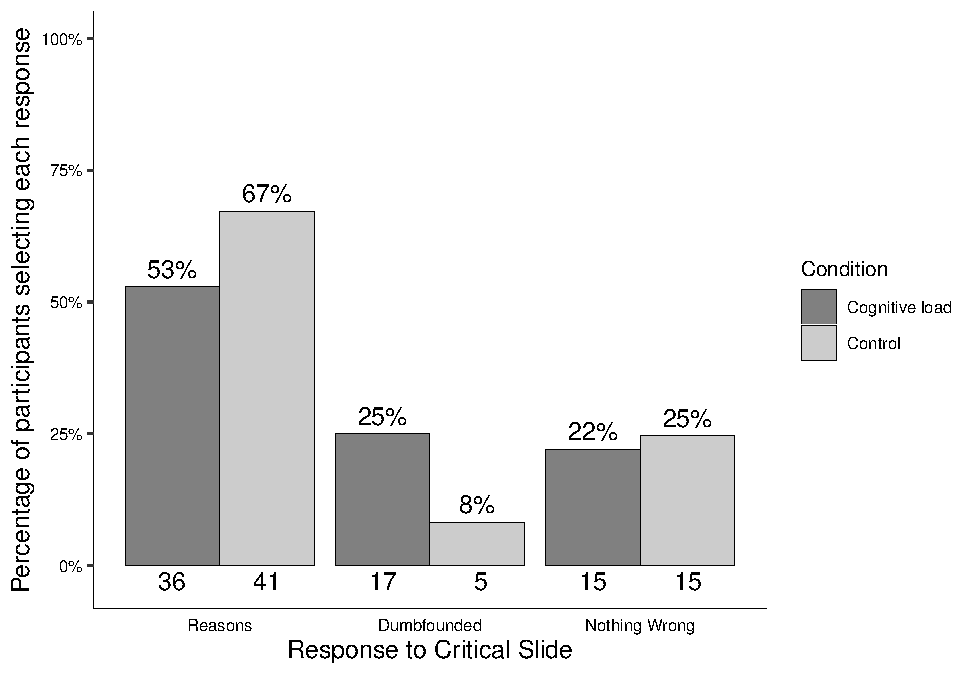
\includegraphics{Study_3_files/figure-latex/S3ch5S3fig2criticalcondition-1.pdf}
\caption{\label{fig:S3ch5S3fig2criticalcondition}Study 3: Responses to critical slide for the cognitive load group (\emph{N} = 68) and the control group (\emph{N} = 61)}
\end{figure}

\begin{table}[tbp]

\begin{center}
\begin{threeparttable}

\caption{\label{tab:S3S3tab1dumb}Study 3 – Observed counts, expected counts, and standardised residuals for each response to the critical slide depending on cognitive load}

\begin{tabular}{llcc}
\toprule
 & \multicolumn{1}{c}{} & \multicolumn{1}{c}{Cognitive Load} & \multicolumn{1}{c}{Control}\\
\midrule
Observed count & Reasons & 36 & 41\\
 & Dumbfounded & 17 & 5\\
 & Nothing Wrong & 15 & 15\\
Expected count & Reasons & 40.59 & 36.41\\
 & Dumbfounded & 11.6 & 10.4\\
 & Nothing Wrong & 15.81 & 14.19\\
Standardised residuals & Reasons & -1.65 & 1.65\\
 & Dumbfounded & 2.53* & -2.53*\\
 & Nothing Wrong & -0.34 & 0.34\\
\bottomrule
\addlinespace
\end{tabular}

\begin{tablenotes}[para]
\normalsize{\textit{Note.} * = sig. at \emph{p} < .05; ** = sig. at \emph{p} < .001}
\end{tablenotes}

\end{threeparttable}
\end{center}

\end{table}

A chi-squared test for independence revealed a significant association between experimental condition and response to the critical slide, \(\chi\)\textsuperscript{2}(2, \emph{N} = 129) = 6.51, \emph{p} = .039, \emph{V} = 0.22, the observed power was 0.62. The responses to the critical slide for the experimental group (\emph{N} = 68) and the control group (\emph{N} = 61) are displayed in Figure~\ref{fig:S3ch5S3fig2criticalcondition}. The observed counts, expected counts and standardised residuals are displayed in Table~\ref{tab:S3S3tab1dumb}.

\newpage

A multinomial logistic regression revealed a significant association between Need for Cognition and response to the critical slide, \(\chi\)\textsuperscript{2}(2, \emph{N} = 129) = 6.43, \emph{p} = .040, the observed power was 0.62. Need for Cognition explained between 2.80\% (Cox and Snell R square) and 3.78\% (Nadelkerke R squared) of the variance in responses to the critical slide. As Need for Cognition increased, participants were significantly more likely to provide reasons than to present as dumbfounded, Wald = 6.08, \emph{p} = .014, odds ratio = 0.69, 95\% CI {[}0.51, 0.93{]} (see Supplementary Analyses Figure XX for relative probabilities of selecting each response depending on Need for Cognition).

\hypertarget{refs}{}
\begin{CSLReferences}{1}{0}
\leavevmode\hypertarget{ref-cacioppo_need_1982}{}%
Cacioppo, J. T., \& Petty, R. E. (1982). The need for cognition. \emph{Journal of Personality and Social Psychology}, \emph{42}(1), 116--131. \url{https://doi.org/10.1037/0022-3514.42.1.116}

\leavevmode\hypertarget{ref-petty_efficient_1984}{}%
Petty, R. E., Cacioppo, J. T., \& Kao, C. F. (1984). The efficient assessment of need for cognition. \emph{Journal of Personality Assessment}, \emph{48}(3), 306--307.

\end{CSLReferences}


\end{document}
